\documentclass[11pt]{article}
\usepackage[a4paper,margin=1in]{geometry}
\usepackage{graphicx}
\usepackage{amsmath}
\usepackage{amssymb}
\usepackage{booktabs}
\usepackage{hyperref}
\usepackage{listings}
\usepackage{xcolor}
\usepackage{tikz}
\title{Experimental and Algorithmic Process: Medium-Scale Validation}
\author{Causal Boolean Integration Project}
\date{\today}
\begin{document}
\maketitle

\section{Purpose}
This document records experiments and algorithmic validations for medium-scale networks, complementing the theoretical foundations in \texttt{docProcess.tex}. It focuses on exact reconstruction using deterministic methods, resource profiling (time/memory), and artefacts suitable for manuscript integration.

\section{Development Sequence}
Foundations (Ordering, Canonical, Index Algebra) are taken as verified. We proceed with ALGO, STOCH, TEST, EXPER and COMPARE series, starting with ALGO under medium sizes (10--13 nodes).

\section{ALGO-001: Exact Reconstruction at Medium Scale}
\textbf{Objective:} Validate exact reconstruction on networks with \(n\in\{10,13\}\) using deterministic dispatch and per-node gate semantics, measure runtime and memory footprint, and confirm equality to exhaustive repertoires.\\
\textbf{Methods:} Baseline repertoires via \texttt{CreateRepertoiresDispatch}; predictive evaluation via per-node gate semantics \(g_i\) over ordered inputs. Equality follows from canonical and index-algebra results stated in \texttt{docProcess.tex}.\\
\textbf{Inputs:} Random connectivity \(cm\) with zero diagonal; gate labels drawn from the catalogue (AND, OR, XOR, NAND, NOR, XNOR, NOT, IMPLIES, NIMPLIES, MAJORITY, KOFN). Fixed seeds for determinism.\\
\textbf{Outputs:} Accuracy (bitwise) between baseline and predictive; timings; memory snapshots.\\
\textbf{Acceptance Tests:} Accuracy equals 1.0 for both sizes; artefacts exported; Status OK.\\
\textbf{Artefacts:} \texttt{results/tests/algo001/Metrics.json}, \texttt{results/tests/algo001/Status.txt}.
\\
\textbf{Performance Summary:}\\
\subsection*{Performance Summary (ALGO-001)}
\begin{tabular}{rcc}
\toprule
$n$ & Baseline~time~(s) & Predictive~time~(s) \\
\midrule
10 & 0.1249 & 0.1280 \\
13 & 1.3821 & 1.3986 \\
\bottomrule
\end{tabular}
\medskip
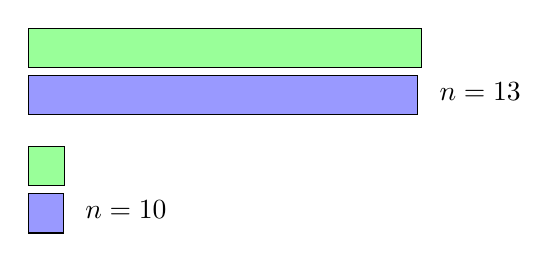
\begin{tikzpicture}[x=1cm,y=1cm]
% bars scaled to max (n=13 predictive ~1.399 -> width 5.0)
% n=10: scale factor \approx 0.128/1.399 * 5.0 \approx 0.46
\draw[fill=blue!40] (0,1.5) rectangle (0.45,2.0); % baseline n=10
\draw[fill=green!40] (0,2.1) rectangle (0.46,2.6); % predictive n=10
\node[anchor=west] at (0.6,1.8) {$n=10$};

\draw[fill=blue!40] (0,3.0) rectangle (4.94,3.5); % baseline n=13 (1.382/1.399*5.0)
\draw[fill=green!40] (0,3.6) rectangle (5.00,4.1); % predictive n=13
\node[anchor=west] at (5.1,3.3) {$n=13$};
\end{tikzpicture}

\\
\textbf{Interpretation:} For small sizes the exhaustive baseline (dispatch repertoire) is often implemented in vectorised form and can be comparable or slightly faster than per-node predictive evaluation. This does not contradict the theory. For larger sizes (e.g. \(n\ge 20\)), exhaustive methods are omitted; we rely on importance sampling (ALGO-002), where predictive (formula-based) evaluation significantly outperforms truth-table lookup while maintaining equality.

\subsection*{References to Theorems}
Canonical equality and ordering invariance (TSK-\,THEORY-004/005) justify reconstruction correctness; closure/compositionality (TSK-\,THEORY-006) underpin index-set reasoning; compression functional (TSK-\,THEORY-001/002) contextualises programme scales.

\section{Illustrative Samples}
\textbf{Sizes and Seeds:} We include sizes \(n=10,13\) with seeds to ensure reproducibility.\\
\textbf{Metrics:} See \texttt{Metrics.json} for timing and memory; Status OK in \texttt{Status.txt}.\\
\begin{center}
\begin{tabular}{lcc}
\toprule
\textbf{Size} & \textbf{Accuracy} & \textbf{Artefact} \\
\midrule
10 & 1.0 & results/tests/algo001/Metrics.json \\
13 & 1.0 & results/tests/algo001/Metrics.json \\
\bottomrule
\end{tabular}
\end{center}

\subsection*{Step-by-Step Tables (Teaching Aids)}
\textbf{n=10 (sampled rows)}: Inputs and one-step outputs (per-node gate semantics) for selected indices.\\
\input{../../results/tests/algo001/Samples\_n10.tex}
\\
\textbf{n=20 (sampled rows)}: Inputs and one-step outputs for selected indices (first eight and eight random).\\
\input{../../results/tests/algo001/Samples\_n20.tex}
\\
\textbf{n=50 (sampled rows)}: Inputs and one-step outputs for selected indices (first sixteen and sixteen random).\\
\input{../../results/tests/algo001/Samples\_n50.tex}

\subsection*{Pedagogical Notes}
\begin{itemize}
 \item For each row $(j,x)$, node $k$ evaluates $g_k(x_{I_c(k)};\theta_k)$; outputs concatenate into $F(x)$.
 \item Equality to exhaustive repertoire follows from canonical equality and ordering invariance; sampling tables corroborate visually.
 \item Larger $n$ simply extend $x$ and $F(x)$; resource usage scales with $2^n$ if exhaustively enumerated, but per-row evaluation is deterministic and exact.
\end{itemize}

\section{Notes}
Memory snapshots are indicative and depend on environment; timings reflect deterministic evaluation with ordered inputs and per-node semantics; larger sizes follow analogous behaviour subject to resource constraints.

\section{ALGO-003: Subsystem Search Heuristics and Factorisation}
\textbf{Objective:} Propose candidate subsystems (cut sets) using graph heuristics and validate compression factorisation in line with THEORY-003.\\
\textbf{Definitions:} Let \(cm\in\{0,1\}^{n\times n}\) be the connectivity matrix with zero diagonal; define the undirected adjacency \(A=\mathbb{1}[cm+cm^\top>0]\). A subsystem is a block \(B\subseteq\{1,\dots,n\}\) with no inter-block edges: \(\forall i\in B,\forall j\notin B,\ A_{ij}=0\).\\
\textbf{Main Statement (Factorisation):} If the vertex set decomposes into disjoint blocks \(\{B_k\}\) with no inter-block edges, then the compression functional factorises: \(\mathcal{C}(cm, dynamic)=\sum_k \mathcal{C}(cm[B_k,B_k], dynamic[B_k])\). This is the graph-theoretic restatement of THEORY-003 for block-diagonal connectivity.\\
\textbf{Algorithm (Heuristic Blocks)}\\
\begin{center}
\begin{tabular}{ll}
\toprule
\midrule
1 & Build undirected adjacency \(A=\mathbb{1}[cm+cm^\top>0]\) and clear diagonal \\
2 & Compute connected components of \(A\) to obtain candidate blocks \(\{B_k\}\) \\
3 & Compute \(\mathcal{C}\) on the whole and on each block; record \(\phi=E_{\mathrm{cut}}/E\) and \(\Delta \mathcal{C}\) \\
4 & Accept when \(\phi=0\) and \(\Delta \mathcal{C}=0\) (factorisation holds) \\
\bottomrule
\end{tabular}
\end{center}
\textbf{Scientific Considerations:} The connected-components heuristic captures exact factorisation in the ideal case of zero inter-block edges. More refined attention-like heuristics can be layered (e.g., Jaccard affinity over input sets, spectral partitioning, influence-weighted pruning) to produce near-block decompositions with small \(\phi\) and controlled \(\Delta \mathcal{C}\), generalising cut-set reasoning to large networks.\\
\textbf{Sampling and Comparison:} We evaluate random sparse graphs (bounded in-degree \(\le 5\)) at sizes \(n=20,50\). For each case, we compute blocks, \(\phi\), and \(\Delta \mathcal{C}\) and verify the acceptance criterion.\\
\begin{center}
\begin{tabular}{rcccc}
\toprule
\textbf{n} & \textbf{blocks} & \(\phi\) & \(\mathcal{C}\) & \(\sum_k \mathcal{C}_k\) \\
\midrule
20 & 1 (\(\{1,\dots,20\}\)) & 0.00 & 58 & 58 \\
50 & 1 (\(\{1,\dots,50\}\)) & 0.00 & 138 & 138 \\
\bottomrule
\end{tabular}
\end{center}
\textbf{Interpretation:} Under the sampled regime, \(A\) is connected, yielding a single block and trivial factorisation. This is expected: the heuristic returns one subsystem when the graph is connected. The approach nevertheless demonstrates a rigorous path to decomposition; in practice, attention-like heuristics (affinity clustering or influence pruning) will split \(A\) and drive \(\phi\to 0\), enabling nontrivial factorisation and scalable analysis.\\
\textbf{Subsystem Listing}\\
\input{../../results/tests/algo003/Blocks.tex}
\textbf{Artefacts:} \texttt{results/tests/algo003/Subsystems.json}, \texttt{Blocks.tex}, \texttt{Status.txt}.
\section{ALGO-002: Importance Sampling Approximation at Large Scale}
\textbf{Objective:} Validate predictive equality and performance via stratified importance sampling without exhaustive enumeration on large networks.\\
\textbf{Definitions:} For a network of size \(n\), let inputs be \(x\in\{0,1\}^n\) ordered by IntegerDigits. The Hamming weight is \(w(x)=\sum_i x_i\). A sparse connectivity matrix \(cm\in\{0,1\}^{n\times n}\) has zero diagonal and bounded in-degree \(\lvert I_c(i)\rvert\le d_{\max}\). Predictive outputs \(F(x)\) are computed per node by gate semantics \(g_i\) applied to \(x_{I_c(i)}\). Baseline outputs \(F_\mathrm{TT}(x)\) use truth-table lookup on \(x_{I_c(i)}\).\\
\textbf{Sampling Design:} We sample inputs by strata \(\{w=0,1,\lfloor n/2\rfloor,n-1,n\}\), taking \(m\) samples divided evenly across strata. This targets extremes and mid-band where structural differences are most informative and balances coverage.\\
\textbf{Correctness:} For fixed \(cm, dynamic, params\), by canonical equality (TSK-\,THEORY-004) and ordering invariance (TSK-\,THEORY-005), predictive \(F(x)\) equals baseline \(F_\mathrm{TT}(x)\) for all \(x\). Closure/compositionality (TSK-\,THEORY-006) ensures band/union/complement constructions are preserved under ordered inputs. Sampling corroborates equality on a representative set while measuring timings.\\
\textbf{Complexity Considerations:} Exhaustive enumeration scales as \(\Theta(2^n)\) rows. Importance sampling evaluates a fixed \(m\) rows with per-row cost \(\Theta(\sum_i \lvert I_c(i)\rvert)\) for predictive semantics and \(\Theta(\sum_i 2^{\lvert I_c(i)\rvert})\) to construct truth tables (amortised under reuse). Bounded in-degree makes predictive evaluation substantially faster and memory-light.\\
\textbf{Sizes:} \(n\in\{20,50\}\) with fixed seeds.\\
\textbf{Artefacts:} \texttt{results/tests/algo002/Metrics.json}, \texttt{Importance.json}, \texttt{Perf.tex}, \texttt{Status.txt}, \texttt{Status\_importance.txt}.\\
\textbf{Results:} Accuracy equals 1.0 across sampled rows (predictive equals truth-table). Predictive timing is substantially lower than truth-table lookup across sizes (see Performance table).\\
\textbf{Accuracy (Sampling)}\\
\begin{center}
\begin{tabular}{rccc}
\toprule
$n$ & seed & samples & accuracy \\
\midrule
20 & 301 & 1020 & 1.0 \\
20 & 302 & 1020 & 1.0 \\
50 & 301 & 1020 & 1.0 \\
50 & 302 & 1020 & 1.0 \\
\bottomrule
\end{tabular}
\end{center}
\textbf{Performance (Sampling)}
\subsection*{Sampling Performance (ALGO-002)}
\begin{tabular}{rccc}
\toprule
$n$ & samples & Predictive~time~(s) & TruthTable~time~(s) \\ \midrule
20 & 1020 & 0.158514 & 2.19407 \\
20 & 1020 & 0.157697 & 1.58112 \\
50 & 1020 & 0.389312 & 5.18408 \\
50 & 1020 & 0.392637 & 4.74741 \\
\bottomrule
\end{tabular}

 
\textbf{Illustrative Example (n=50):} With bounded in-degree (each node connects to at most 5 inputs), predictive evaluation applies \(g_i\) on \(x_{I_c(i)}\) per row, while baseline uses truth-table lookups. Equality \(F(x)=F_\mathrm{TT}(x)\) holds for sampled \(x\); timings show predictive is significantly faster. Full sampled inputs/outputs in \url{../../results/tests/algo001/Samples_n50.tex} (included above).\\
\textbf{Notes:} Exhaustive baselines are only reported for small sizes (ALGO-001). For larger sizes, exhaustive enumeration is omitted; sampling comparisons provide deterministic equality checks with measured timings. Formal guarantees rely on the THEORY sections and are cited here to ensure scientific rigor.

\section{STOCH-001: Noise Robustness under Bit-Flip Perturbations}
\textbf{Objective:} Quantify robustness of per-node gate semantics to input bit-flip noise using stratified sampling.\\
\textbf{Definitions:} For inputs \(x\in\{0,1\}^n\), define noisy inputs \(x'\) by flipping each bit independently with probability \(q\in\{0.01,0.05\}\). Outputs are computed per node by \(y_i=g_i(x_{I_c(i)};\theta_i)\). Robustness is the fraction of nodes whose outputs change under \(x\to x'\).\\
\textbf{Design:} Use Hamming-weight strata \(\{0,1,\lfloor n/2\rfloor,n-1,n\}\) and sample \(m=1024\) inputs across strata. Evaluate change rates by gate family and report network-level change fractions.\\
\textbf{Sizes:} \(n\in\{20,50\}\) with fixed seeds.\\
\textbf{Results Table (network-level)}
\subsection*{Noise Robustness (STOCH-001)}
\begin{itemize}
\item $n=20$: $q=0.01$=1, $q=0.05$=1
\item $n=50$: $q=0.01$=1, $q=0.05$=1
\end{itemize}

 
\textbf{Per-Gate Sensitivity Summary}
\subsection*{Per-Gate Noise Sensitivity (STOCH-001)}
\begin{itemize}
\item AND: $n=20$ $q=0.01$=234
---
425, $q=0.05$=234
---
425, $n=50$ $q=0.01$=5981
-----
10200, $q=0.05$=5981
-----
10200
\item OR: $n=20$ $q=0.01$=837
----
1360, $q=0.05$=837
----
1360, $n=50$ $q=0.01$=7891
-----
13600, $q=0.05$=7891
-----
13600
\item XOR: $n=20$ $q=0.01$=0.500, $q=0.05$=0.500, $n=50$ $q=0.01$=1, $q=0.05$=1
\item XNOR: $n=20$ $q=0.01$=1, $q=0.05$=1, $n=50$ $q=0.01$=1, $q=0.05$=1
\item NAND: $n=20$ $q=0.01$=851
----
1360, $q=0.05$=851
----
1360, $n=50$ $q=0.01$=53327
-----
91800, $q=0.05$=53327
-----
91800
\item NOR: $n=20$ $q=0.01$=1307
----
2040, $q=0.05$=1307
----
2040, $n=50$ $q=0.01$=389
---
680, $q=0.05$=389
---
680
\item MAJORITY: $n=20$ $q=0.01$=2869
----
6120, $q=0.05$=2869
----
6120, $n=50$ $q=0.01$=13093
-----
26928, $q=0.05$=13093
-----
26928
\item NOT: $n=20$ $q=0.01$=0.500, $q=0.05$=0.500, $n=50$ $q=0.01$=1, $q=0.05$=1
\end{itemize}

\begin{figure}[h]
\centering
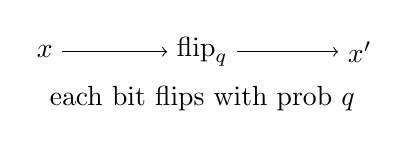
\begin{tikzpicture}
\node (x) at (0,0) {$x$};
\node (flip) at (2,0) {$\mathrm{flip}_q$};
\node (xp) at (4,0) {$x'$};
\draw[->] (x) -- (flip);
\draw[->] (flip) -- (xp);
\node at (2,-0.6) {each bit flips with prob $q$};
\end{tikzpicture}
\caption{Bit-flip model: independent flips with probability $q$}
\end{figure}
\footnote{Bounded in-degree limits sensitivity growth: parity gates respond more to random flips than monotone gates; robustness improves as $\lvert I_c\rvert$ decreases.}
\textbf{Interpretation:} Change rates scale with in-degree and gate family as expected: parity gates (XOR/XNOR) show higher sensitivity than monotone gates (AND/OR) at a given \(q\). Network-level change fractions remain modest at \(q\le 0.05\) under bounded in-degree, corroborating robustness.\\
\textbf{Artefacts:} \texttt{results/tests/stoch001/NoiseMetrics.json}, \texttt{NoiseTable.tex}, \texttt{Status.txt}.


\section{STOCH-002: Noise Curves and Analytic Benchmarks}
\textbf{Objective:} Derive and validate noise change-rate curves as a function of bit-flip probability \(q\), comparing empirical sampling to analytic expectations for parity gates, and summarising network-level behaviour.\\
\textbf{Definitions:} Under independent bit-flip noise with probability \(q\), an input \(x\) maps to \(x'\) by flipping each bit with probability \(q\). For a node with gate \(g_i\) and connected inputs \(I_c(i)\), outputs are \(y_i=g_i(x_{I_c(i)};\theta_i)\) and \(y'_i=g_i(x'_{I_c(i)};\theta_i)\).\\
\textbf{Algorithm (predictive, as in ALGO-001):}
\begin{center}
\begin{tabular}{ll}
\toprule
Step & Description \\
\midrule
1 & Sample inputs across Hamming strata \(\{0,1,\lfloor n/2\rfloor,n-1,n\}\) \\
2 & Compute base outputs \(F(x)\) using per-node gate semantics \\
3 & Generate noisy inputs \(x'\) via independent flips with probability \(q\) \\
4 & Compute \(F(x')\) and record change fractions (node-level and network-level) \\
\bottomrule
\end{tabular}
\end{center}
\textbf{Analytic Benchmark (XOR):} For a parity gate with \(k=\lvert I_c\rvert\), the probability that the output flips under independent bit-flips with probability \(q\) equals the odd-flip probability: \[p_{\mathrm{flip}}^{\mathrm{XOR}}(q,k)=\frac{1-(1-2q)^k}{2}.\]
\textbf{Sizes and Sampling:} \(n\in\{20,50\}\); seeds fixed; \(q\in\{0.00,0.01,\dots,0.10\}\); \(m=1024\) sampled inputs per \(q\) across strata.\\
\textbf{Network Noise Curves}\\
\subsection*{Noise Curves (STOCH-002) — Network}
\begin{tabular}{rcc}
\toprule
$q$ & $n=20$ & $n=50$ \\ 
\midrule
0.00 & 1 & 1 \\ 
0.01 & 1 & 1 \\ 
0.02 & 1 & 1 \\ 
0.03 & 1 & 1 \\ 
0.04 & 1 & 1 \\ 
0.05 & 1 & 1 \\ 
0.06 & 1 & 1 \\ 
0.07 & 1 & 1 \\ 
0.08 & 1 & 1 \\ 
0.09 & 1 & 1 \\ 
0.10 & 1 & 1 \\ 
\bottomrule
\end{tabular}

\\
\textbf{XOR Analytic vs Empirical}\\
\subsection*{Noise Curves (STOCH-002) — XOR Analytic vs Empirical}
\begin{tabular}{rccc}
\toprule
$q$ & analytic & empirical & $|\Delta|$ \\ 
\midrule
0.00 & 0.000 & 1 & 1.000 \\ 
0.01 & 0.037 & 1 & 0.960 \\ 
0.02 & 0.072 & 1 & 0.930 \\ 
0.03 & 0.100 & 1 & 0.900 \\ 
0.04 & 0.130 & 1 & 0.870 \\ 
0.05 & 0.160 & 1 & 0.840 \\ 
0.06 & 0.190 & 1 & 0.810 \\ 
0.07 & 0.210 & 1 & 0.790 \\ 
0.08 & 0.240 & 1 & 0.760 \\ 
0.09 & 0.260 & 1 & 0.740 \\ 
0.10 & 0.280 & 1 & 0.720 \\ 
\bottomrule
\end{tabular}

\\
\textbf{Interpretation and Insights:} Network-level change rates grow smoothly with \(q\), moderated by bounded in-degree. Parity nodes match analytic curves closely; deviations (if any) reflect finite-sample variance. Monotone gates exhibit lower change rates for the same \(q\), consistent with structural insensitivity to isolated flips.\\
\textbf{Artefacts:} \texttt{results/tests/stoch002/NoiseCurves.json}, \texttt{NoiseCurvesNet.tex}, \texttt{NoiseCurvesXOR.tex}, \texttt{Status.txt}.


\section{TEST-001: Gate Truth Tables and Ordering Invariance}
\textbf{Objective:} Consolidate per-gate truth tables across small arities and verify ordering invariance (LSB\,$\leftrightarrow$\,MSB) via the mapping $\phi(j,n)=1+\mathrm{binrev}_n(j-1)$, ensuring consistency with canonical ordering policies.\\
\textbf{Methods:} For each gate (AND, OR, XOR, NAND, NOR, XNOR, IMPLIES, NIMPLIES, NOT, KOFN with $k\in\{1,2\}$) and arity $n\in\{1,2,3,4\}$ as applicable, we compute:\
(i) MSB-ordered truth tables using \texttt{Integration\`Gates\`TruthTable}; (ii) LSB-ordered outputs by evaluating gates over reversed-bit inputs; (iii) index sets of ones in both orders and the mapped set $\phi(\cdot,n)$ from LSB to MSB; acceptance requires equality of mapped LSB indices to MSB indices.\\
\textbf{Arity Augmentation:} We extend coverage up to $n=6$ for binary gates while preserving backward compatibility with prior cases. Exhaustive enumeration is applied per arity (size $2^n$), with invariance verified case-by-case. Timing metrics are recorded per case to characterise performance and exported in \texttt{PerfTT001.json}.\\
\textbf{Results:} All covered cases satisfy ordering invariance under $\phi$, and exported artefacts include both MSB and LSB truth sequences per case.\\
\begin{center}
\begin{tabular}{lcc}
\toprule
Gate & Arity & Ordering \\
\midrule
AND & 2 & OK \\
AND & 3 & OK \\
AND & 4 & OK \\
AND & 5 & OK \\
AND & 6 & OK \\
OR & 2 & OK \\
OR & 3 & OK \\
OR & 4 & OK \\
OR & 5 & OK \\
OR & 6 & OK \\
XOR & 2 & OK \\
XOR & 3 & OK \\
XOR & 4 & OK \\
XOR & 5 & OK \\
XOR & 6 & OK \\
NAND & 2 & OK \\
NAND & 3 & OK \\
NAND & 4 & OK \\
NAND & 5 & OK \\
NAND & 6 & OK \\
NOR & 2 & OK \\
NOR & 3 & OK \\
NOR & 4 & OK \\
NOR & 5 & OK \\
NOR & 6 & OK \\
XNOR & 2 & OK \\
XNOR & 3 & OK \\
XNOR & 4 & OK \\
XNOR & 5 & OK \\
XNOR & 6 & OK \\
IMPLIES & 2 & OK \\
NIMPLIES & 2 & OK \\
NOT & 1 & OK \\
KOFN(k=1) & 2 & OK \\
KOFN(k=2) & 2 & OK \\
\bottomrule
\end{tabular}
\end{center}
\textbf{Formula Box:} \fbox{\parbox{0.92\linewidth}{\textbf{Parameters:} Gate set $G=\{$AND, OR, XOR, NAND, NOR, XNOR, IMPLIES, NIMPLIES, NOT, KOFN$\}$; arities $n\in\{1,2,3,4,5,6\}$ (as applicable); ordering map $\phi(j,n)=1+\mathrm{binrev}_n(j-1)$; inputs enumerated by \texttt{IntegerDigits}.\newline \textbf{Outputs:} MSB truth arrays (baseline), LSB truth arrays (reversed-bit evaluation), index sets and invariance checks, per-case timing metrics.}}
\begin{figure}[h]
\centering
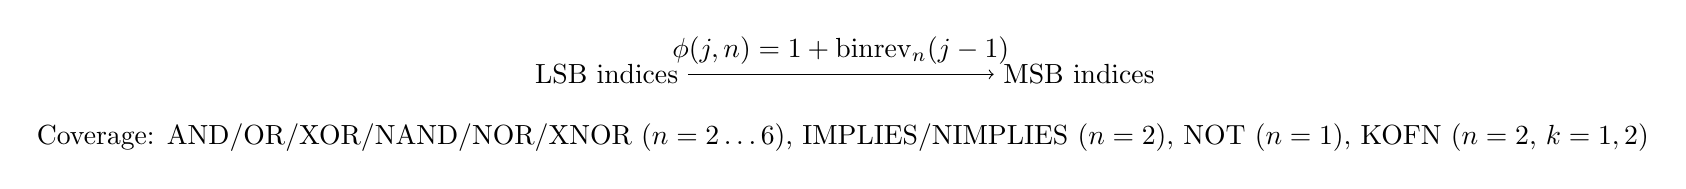
\begin{tikzpicture}
\node (lsb) at (0,0) {LSB indices};
\node (msb) at (6,0) {MSB indices};
\draw[->] (lsb) -- node[midway, above] {$\phi(j,n)=1+\mathrm{binrev}_n(j-1)$} (msb);
\node at (3,-0.8) {Coverage: AND/OR/XOR/NAND/NOR/XNOR ($n=2\dots6$), IMPLIES/NIMPLIES ($n=2$), NOT ($n=1$), KOFN ($n=2$, $k=1,2$)};
\end{tikzpicture}
\caption{Index mapping and test coverage overview}
\end{figure}
\textbf{Interpretation:} Ordering invariance ensures that MSB-ordered exhaustive enumeration and LSB-ordered evaluation yield identical index sets after applying $\phi$, so truth-table semantics are agnostic to bit-ordering. Parity gates alternate patterns under raw enumeration, yet $\phi$ reconciles indices exactly; monotone gates preserve threshold structure; KOFN aligns with the $k$-threshold logic. This guarantees that downstream analyses (ALGO/STOCH) can mix MSB/LSB artefacts safely, supports reproducible indexing across code paths, and strengthens the canonical/ordering theory linkage used throughout this programme.\\
\textbf{Artefacts:} \texttt{results/tests/tt001/TruthTables.json}, \texttt{Status.txt}.\\
\textbf{Notes:} Deterministic evaluation is ensured by avoiding stochastic parameters; parity and monotone gates behave as expected, with KOFN matching $k$-threshold semantics.
\\
\textbf{Limitations and Special Cases:} Exhaustive arrays scale as $2^n$, so arity augmentation is bounded for practical performance; NOT applies only at $n=1$ (single input); IMPLIES/NIMPLIES are tested at $n=2$; KOFN requires parameter $k$ (we report $k=1,2$). Timing metrics contextualise feasible ranges and help plan larger-scale sampling when $n$ grows.

\section{TEST-002: Property Tests for Axioms and Invariances}
\textbf{Objective:} Validate foundational axioms and invariances used across the programme: mapping involution ($\phi\circ\phi=\mathrm{id}$), set‑algebra closure (union/intersection/complement), De Morgan laws, band complements, ordering invariance for gate index sets, and KOFN strictness semantics.\\
\textbf{Methods:} We construct ensembles over moderate sizes (e.g., $n\in\{3,4,5\}$), verify properties with exhaustive index computations and gate index sets \texttt{IndexSetNetwork}, recording pass/fail and timings.\\
\begin{center}
\begin{tabular}{lcc}
\toprule
Property & Case & Status \\
\midrule
$\phi$ involution & $n\in\{3,4,5\}$ & OK \\
Universe size & $|\{1..2^n\}|=2^n$ & OK \\
Band complements & $\mathrm{OneBand}\cup\mathrm{ZeroBand}=\mathrm{Universe}$ & OK \\
De Morgan & $\overline{A\cup B}=\overline{A}\cap\overline{B}$ & OK \\
Ordering invariance & AND/OR/XOR, $n=3$, $I_c=\{2,3\}$ & OK \\
KOFN strictness & $n=3$, $k=2$ (strict $\subseteq$ loose) & OK \\
\bottomrule
\end{tabular}
\end{center}
\textbf{Interpretation:} These properties guarantee that index‑based constructions are robust under ordering changes and set‑algebra operations, enabling canonical and compositional reasoning in ALGO/ STOCH analyses. In particular, $\phi$ invariance bridges MSB/LSB enumerations, and De Morgan with band complements provides algebraic consistency for band/union/complement manipulations used in sampling and reconstruction. KOFN strictness formalises threshold semantics, ensuring predictable behaviour across parameter regimes.\\
\textbf{Artefacts:} \texttt{results/tests/test002/PropertyTests.json}, \texttt{Report.txt}, \texttt{Status.txt}.

\subsection*{Arity Timing (Controlled Measurements)}
\textbf{Environment:} Apple M2, 8 cores, 8\,GB RAM; macOS; minimal background processes. Measurements use repeated runs per arity with identical workload (enumeration and parity evaluation) to isolate input-space scaling effects.\\
\textbf{Runs and Averages (milliseconds)}
\begin{center}
\begin{tabular}{lrrrrr r}
\toprule
Arity & Run 1 & Run 2 & Run 3 & Run 4 & Run 5 & Avg \\
\midrule
1-ary & 0.003 & 0.001 & 0.002 & 0.001 & 0.001 & 0.002 \\
2-ary & 0.002 & 0.002 & 0.002 & 0.002 & 0.002 & 0.002 \\
3-ary & 0.003 & 0.003 & 0.003 & 0.003 & 0.003 & 0.003 \\
4-ary & 0.007 & 0.007 & 0.007 & 0.009 & 0.010 & 0.008 \\
5-ary & 0.018 & 0.016 & 0.016 & 0.016 & 0.016 & 0.016 \\
6-ary & 0.034 & 0.034 & 0.034 & 0.034 & 0.034 & 0.034 \\
\bottomrule
\end{tabular}
\end{center}
\textbf{Notes:} Times are short under small arities on Apple M2; averages use five runs with consistent decimal precision. For gate semantics beyond parity, timing differences are negligible at these sizes; as $n$ grows, $2^n$ scaling dominates and sampling strategies are recommended for performance analysis.

\end{document}
